En este capítulo se desarollará el estudio económico del proyecto llevado a cabo en el Centro de Salud de Laguna de Duero.
Para ello, se desglosará su elaboración en las distintas fases que lo componen, desde la propuesta de realización hasta la redacción del informe final.
Para su valoración, se tienen en cuenta las horas dedicadas de los distintos participantes además de los recursos tanto directos como indirectos empleados en las distintas fases.

\section{Profesionales involucrados}

Para la realización de este proyecto ha sido necesaria la participación de distintos profesionales del sector sanitario.
En primer lugar, se encuentra el Subdirector de Gestión y SSGG del Área de Salud Valladolid Oeste que actúa de promotor del proyecto.
Es el responsable de que el proyecto se lleve a cabo además de coordinar y aconsejar en los distintas situaciones.
Será el encargado de la aprobación y validación final del proyecto.

Seguidamente, se encuentra el Ingeniero Industrial que llevará a cabo toda las tareas de recopilación de información y documentación del trabajo.
Además, se encarga de organizar y formar el grupo de trabajo del centro.
A partir de sus conocimientos, sobre todo, en organización industrial, realizará las tareas de análisis y síntesis de los procesos principales de la sección administrativa del centro.

Finalmente, se encuentran los administrativos que forman el grupo de trabajo del proyecto.
Se encargan de ofrecer toda la información necesaria sobre sus labores además de exponer las distintas dificultades con las que se encuentran en su día a día.
Además, pueden proponer distintas mejoras y soluciones a las problemáticas analizadas en el propio proyecto.

\section{Fases del proyecto}

Conocer las fases del proyecto es necesario para estimar los costes económicos asociados a cada fase.
A continuación, se describen las fases en las que se ha desarollado el proyecto.
Además, en la Figura~\ref{fig:gantt} se muestra de forma visual la planificación del proyecto en base a un diagrama de Gantt.

\begin{figure}[H]
    \centering
    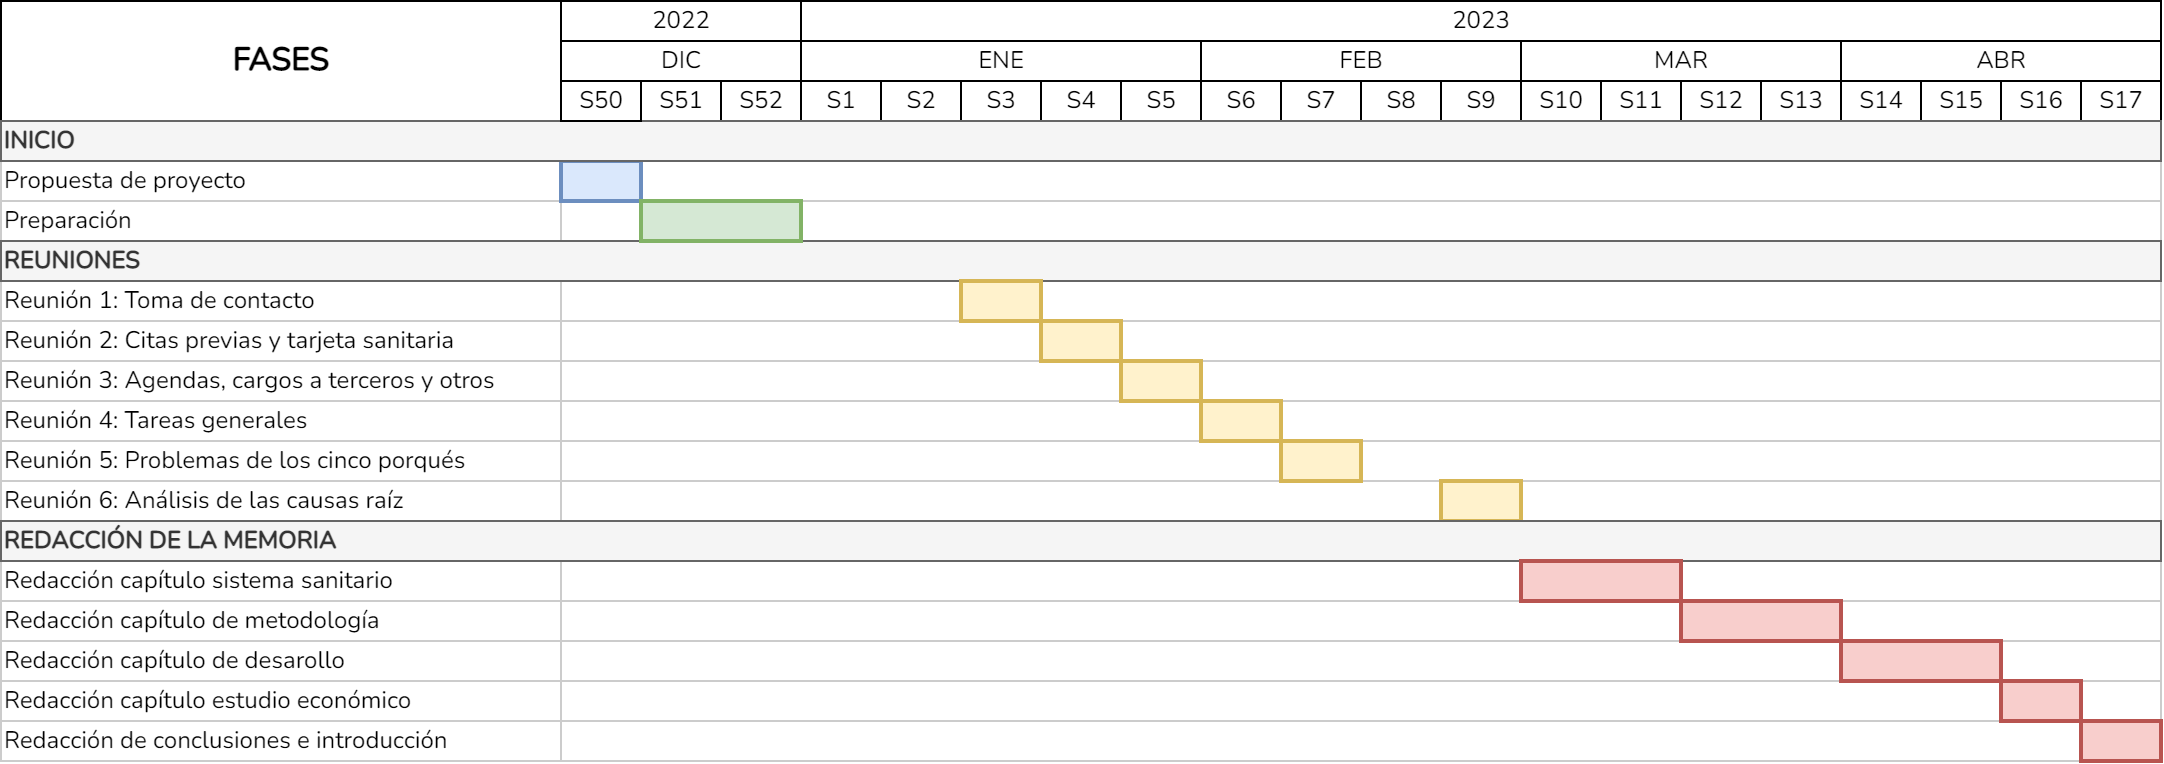
\includegraphics[width=\textwidth]{img/gantt-diagram.png}
    \caption{Diagrama de Gantt del proyecto}
    \label{fig:gantt}
\end{figure}

\subsection{Propuesta de elaboración de proyecto}

El proyecto comienza con la propuesta por parte de la Subdirección de Gestión del Área de Salud Valladolid Oeste de la realización de un proyecto de aplicación de técnicas de mejora continua a un centro de Atención Primaria.
Es en esta fase donde se elige el centro de Laguna de Duero por ser el mejor representante de los servicios ofrecidos en las distintas Zonas Básicas de Salud.
Además, se exponen los objetivos que se quieren alcanzar, la estandarización de tareas junto con la propuesta de mejoras, junto con la metodología a seguir.

\subsection{Formación del grupo de trabajo}

En esta fase se forma el grupo de trabajo con el que se desarrollará todo el proyecto.
Previamente, fue necesario documentarse en la aplicación de técnicas de mejora continua en entornos de oficina y sanitarios.
Además, en esta fase se preparó una página web en \Gls{sharepoint} que sirvió para poder compartir con todos los miembros del grupo el progreso del trabajo.

\subsection{Recopilación de información}

Una vez formado el grupo, se organizaron reuniones semanales con un grupo pequeño de trabajadores a modo de muestra que conocieran bien su puesto de trabajo para poder recopilar toda la información de las operaciones y tareas llevadas a cabo en la sección.
Se realizaron un total de seis reuniones que se pueden separar en dos fases.
Por un parte las cuatro primeras reuniones se centraron en recoger información de todas las tareas administrativas que se realizan en los puestos administrativos de cara a definir un estándar y, por otras parte, las dos últimas reuniones se centraron en obtener un listado de problemas su posterior análisis de las causas raíz con la técnica de los cinco porqués.

\subsubsection{Reunión 1: Toma de contacto}

En esta primera reunión asistieron los dos subdirectores de gestión del área.
Fue una presentación corta en la que se explicó al grupo de trabajo la necesidad de realizar una estandarización de las tareas administrativas de la sección del centro con el fin de analizar las cargas de trabajo reales.
Además, se propuso el análisis mediante la técnica de los cinco porqués las causas raíz de los problemas administrativos.

\subsubsection{Reunión 2: Citas previas y tarjeta sanitaria}

Dado que la gestión de citas previas era proceso principal de la sección administrativa fue el primero que se trató.
Se explicó con detalle los distintos tipos de citas: consultas generales, pruebas de laboratorio y citas de especialidades.
Además de explicar el proceso, se entregó una copia a modo de ejemplo de los volantes de extracciones y de radiología en los cuales el facultativo especifica qué pruebas concretas se deben de realizar al paciente.

\subsubsection{Reunión 3: Agendas, cargos a terceros, reclamaciones y absentismo}

En esta reunión se trataron los procesos de gestión de agendas, la tramitación de cargos a terceros, reclamaciones y las solicitudes de permisos retribuidos.
En cada uno de ello se ofrecieron los distintos formularios utilizados en cada proceso.

\subsubsection{Reunión 4: Tareas generales}

En esta reunión sobre la estandarización se desarrollaron por parte del personal otras tareas generales que no pertenecen a ninguno de los procesos principales.

\subsubsection{Reunión 5: Listado de problemas para los cinco porqués}

En esta reunión se realizó la presentación y explicación de la herramienta de los cinco porqués con el fin de analizar las causas raíz de los problemas presentes en la sección.
Se realizó un ``brainstorming'' en el que participaron todos los miembros del grupo de trabajo con el fin de definir todos los problemas administrativos.
Posteriormente se filtraron para valorar los que más impacto tenían en el rendimiento del equipo.

\subsubsection{Reunión 6: Análisis de las causas raíz y propuestas de mejora}

En esta última reunión se fueron comentando cada uno de los problemas listados en la anterior reunión a la vez que se aplicaba la ténica de los cinco porqués.
Una vez obtenidos las causas de cada problema, se propusieron posibles soluciones a cada una de las problemáticas.
Finalmente, se discutió la viabilidad de cada una.

\subsection{Redacción de la documentación}

Finalmente, tras recoger todos los datos necesarios se procede a analizar toda la información recopilada y a redactar la memoria del trabajo.

\section{Estimación de costes}

En este apartado se lleva a cabo la valoración económica del proyecto a partir de todos los recursos necesarios para su desarrollo.
En la evaluación económica se tienen en cuenta una relación de los costes asociados a los siguientes apartados: personal, amortizaciones de los  equipos informáticos, materiales consumibles y servicios indirectos del proyecto.
Se analiza cada una de esas partes de forma individual con el objetivo de conocer la influencia que tiene cada una de ellas sobre el valor final del estudio.

\subsection{Horas efectivas anuales y tasas horarias de personal}

En primer lugar obtienen las horas trabajadas anuales de los profesionales implicados.
Dado que todos los profesionales pertenecen al Sacyl las horas trabajadas se corresponden con un total de 35 horas semanales \cite{noauthor_orden_2022}, es decir, \textbf{1533 horas} anuales.
Seguidamente, se calculan los costes horarios (Tabla~\ref{tab:salarios}) acorde a las tablas salariales del año 2023 del Sacyl~\cite{noauthor_orden_2023}.

\begin{table}[H]
    \centering
    \begin{tabular}{llll}
        \toprule
        Concepto                 & Sub. Gestión & Ing. Industrial & Aux. Administativo \\
        \midrule
        Salario                  & € 56,369.32  & € 38,938.06     & € 21,898.88        \\
        Seguridad Social Empresa & € 19,729.26  & € 13,628.32     & € 7,664.61         \\
        \midrule
        Total                    & € 76,098.58  & € 52,566.38     & € 29,563.49        \\
        Coste horario            & € 48.22      & € 33.31         & € 18.73            \\
        \bottomrule
    \end{tabular}
    \caption{Coste salarial de los profesionales participantes}
    \label{tab:salarios}
\end{table}

\subsection{Costes de amortización de equipos informáticos}

En este apartado se han calculado los costes de las amortizaciones de los equipos utilizados en el proyecto.
La amortización es la pérdida de valor que los bienes del inmovilizado de la empresa sufren a medida que se van usando, porque se producen avances con la investigación que hacen que se vayan quedando anticuados o por el mero transcurso del tiempo.
En este caso fue necesario el uso de un ordenador junto con un conjunto de periféricos.
También se incluyen las licencias de los distintos programas informáticos utilizados.

La amortización de estos equipos se ha calculado considerando una vida útil de cinco años tal y como se muestra en las Tablas~\ref{tab:coste-equipos} y \ref{tab:coste-amortizacion}.

\begin{table}[H]
    \centering
    \begin{tabular}{llll}
        \toprule
        Equipo              & Coste      & Cantidad & Coste total \\
        \midrule
        Ordenador HP        & € 783.34   & 1        & € 783.34    \\
        Licencia Windows 10 & € 108.23   & 1        & € 108.23    \\
        Licencia Office 365 & € 127.12   & 1        & € 127.12    \\
        Impresora Kyocera   & € 97.23    & 1        & € 97.23     \\
        \midrule
        Total a amortizar   & € 1,115.92 &          & € 1,115.92  \\
        \bottomrule
    \end{tabular}
    \caption{Coste de amortización en euros de los equipos utilizados}
    \label{tab:coste-equipos}
\end{table}

\begin{table}[H]
    \centering
    \begin{tabular}{lll}
        \toprule
        Tipo    & Número  & Amortización \\
        \midrule
        Diaria  & € 3.06  & € 0.61       \\
        Semanal & € 21.46 & € 4.29       \\
        Horaria & € 0.71  & € 0.14       \\
        \bottomrule
    \end{tabular}
    \caption{Desglose temporal de las amortizaciones }
    \label{tab:coste-amortizacion}
\end{table}

\subsection{Coste de material consumible}

El coste de los consumibles (papeles de impresora, disquetes, CD's, etc.) se ha calculado según su consumo medio, por persona y hora de trabajo como se muestra en la Tabla~\ref{tab:coste-consumibles}.

\begin{table}[H]
    \centering
    \begin{tabular}{ll}
        \toprule
        Consumible                & Coste    \\
        \midrule
        Papel de impresión        & € 63.00  \\
        Suministro de impresión   & € 273.00 \\
        CD y USB                  & € 16.00  \\
        Otros                     & € 37.00  \\
        \midrule
        Coste anual por persona   & € 389.00 \\
        Coste horario por persona & € 0.25   \\
        \bottomrule
    \end{tabular}
    \caption{Costes de material consumible}
    \label{tab:coste-consumibles}
\end{table}

\subsection{Costes indirectos}

El coste indirecto es aquel que afecta al proyecto pero que no puede imputarse a ninguna de las fases o etapas del mismo.
En este caso se hacen referencia a los consumos de electricidad, telefonía, etc.
En la Tabla~\ref{tab:coste-indirecto} se muestran los costes por persona y hora para cada uno de los conceptos.

\begin{table}[H]
    \centering
    \begin{tabular}{ll}
        \toprule
        Concepto                  & Coste    \\
        \midrule
        Teléfono                  & € 63.00  \\
        Electricidad              & € 273.00 \\
        Otros                     & € 146.00 \\
        \midrule
        Coste annual por persona  & € 482.00 \\
        Coste horario por persona & € 0.31   \\
        \bottomrule
    \end{tabular}
    \caption{Costes indirecto}
    \label{tab:coste-indirecto}
\end{table}

\subsection{Tiempos asociados a cada fase del proyecto}

Los costes de personal corresponden a todas las personas implicadas en el proyecto que han dedicado parte de su jornada laboral al mismo.
En la Tabla~\ref{tab:horas-trabajadas} se muestra el reparto de horas trabajadas por cada grupo de personal y por fase de proyecto.
Cabe destacar que en la columna de administrativos se ha tenido en cuenta las horas dedicadas por los cuatro trabajadores de la sección administrativa del centro de salud.

\begin{table}[H]
    \centering
    \begin{tabular}{llllll}
        \toprule
        Personal            & Fase I & Fase II & Fase III & Fase IV & Total \\
        \midrule
        Sub. Gestión        & 1      & 0       & 12       & 0       & 13    \\
        Ing. Industrial     & 8      & 32      & 48       & 212     & 300   \\
        Aux. Administrativo & 0      & 0       & 48       & 0       & 48    \\
        \midrule
        Total               & 9      & 32      & 108      & 212     & 361   \\
        \bottomrule
    \end{tabular}
    \caption{Desglose de horas dedicadas por tipo de profesional y fase}
    \label{tab:horas-trabajadas}
\end{table}

\section{Costes asignados a cada fase del proyecto}

Para calcular los costes asignados a cada fase se tendrán en cuenta todos los costes de amortización, consumibles, indirectos y de personal junto con las horas dedicadas en cada etapa por todos los profesionales.

\subsection{Fase I: Propuesta de elaboración de proyecto}

En esta primera fase tan solo intervienen el Subdirector y el Ingeniero Industrial con el fin de proponer y establecer los objetivos.

\begin{table}[H]
    \centering
    \begin{tabular}{@{}llll@{}}
        \toprule
        Concepto            & Horas & Coste horario & Coste total \\ \midrule
        Sub. Gestión        & 1     & € 48.22       & € 48.22     \\
        Ing. Industrial     & 8     & € 33.31       & € 266.50    \\
        Aux. Administrativo & 0     & € 33.31       & € -         \\
        Amortización        & 197   & € 0.14        & € 27.82     \\
        Consumibles         & 39    & € 0.25        & € 9.70      \\
        Costes indirectos   & 39    & € 0.31        & € 12.02     \\
        \midrule
        Coste total         &       &               & € 364.26    \\
        \bottomrule
    \end{tabular}
    \caption{Costes asociados a la Fase I}
    \label{tab:fase-propuesta}
\end{table}

\subsection{Fase II: Formación del grupo de trabajo}

En esta segunda fase interviene solamente el Ingeniero Industrial en su labor de preparación del grupo y de estudio de la aplicación de las técnicas de mejora continua en el ámbito sanitario.

\begin{table}[H]
    \centering
    \begin{tabular}{llll}
        \toprule
        Concepto            & Horas & Coste horario & Coste total \\
        \midrule
        Sub. Gestión        & 0     & € 48.22       & € -         \\
        Ing. Industrial     & 32    & € 33.31       & € 1,065.98  \\
        Aux. Administrativo & 0     & € 33.31       & € -         \\
        Amortización        & 0     & € 0.14        & € 98.92     \\
        Consumibles         & 140   & € 0.25        & € 34.48     \\
        Costes indirectos   & 140   & € 0.31        & € 42.73     \\
        \midrule
        Coste total         &       &               & € 1,242.11  \\
        \bottomrule
    \end{tabular}
    \caption{Costes asociados a la Fase II}
    \label{tab:fase-formacion}
\end{table}

\subsection{Fase III: Recopilación de información}

En esta tercera intervienen el Ingeniero Industrial junto con los administrativos del grupo de trabajo. En las horas se tienen en cuentan todas las reuniones organizadas.

\begin{table}[H]
    \centering
    \begin{tabular}{llll}
        \toprule
        Concepto            & Horas & Coste horario & Coste total \\
        \midrule
        Sub. Gestión        & 12    & € 48.22       & € 578.70    \\
        Ing. Industrial     & 48    & € 33.31       & € 1,598.98  \\
        Aux. Administrativo & 48    & € 33.31       & € 1,598.98  \\
        Amortización        & 0     & € 0.14        & € 333.85    \\
        Consumibles         & 472   & € 0.25        & € 116.38    \\
        Costes indirectos   & 472   & € 0.31        & € 144.20    \\
        \midrule
        Coste total         &       &               & € 4,371.08  \\
        \bottomrule
    \end{tabular}
    \caption{Costes asociados a la Fase III}
    \label{tab:fase-recopilacion}
\end{table}

\subsection{Fase IV: Redacción de la documentación}

En esta cuarta, y última, fase interviene solamente el Ingeniero Industrial que se encarga de analizar toda la información recopilada y redactar el informe final.

\begin{table}[H]
    \centering
    \begin{tabular}{llll}
        \toprule
        Concepto            & Horas & Coste horario & Coste total \\
        \midrule
        Sub. Gestión        & 0     & € 48.22       & € -         \\
        Ing. Industrial     & 212   & € 33.31       & € 7,062.15  \\
        Aux. Administrativo & 0     & € 33.31       & € -         \\
        Amortización        & 0     & € 0.14        & € 655.33    \\
        Consumibles         & 927   & € 0.25        & € 228.44    \\
        Costes indirectos   & 927   & € 0.31        & € 283.06    \\
        \midrule
        Coste total         &       &               & € 8,228.98  \\
        \bottomrule
    \end{tabular}
    \caption{Costes asociados a la Fase IV}
    \label{tab:fase-redaccion}
\end{table}

\section{Cálculo del coste total}

La estimación del coste total de trabajo de fin de máster se obtiene de la suma de los distintos costes totales de cada una de las partidas definidas en los apartados anteriores.
En la Tabla~\ref{tab:coste-total} se reflejan todos los costes y su peso sobre el total.

\begin{table}[H]
    \centering
    \begin{tabular}{lll}
        \toprule
        Actividad                                       & Horas & Coste       \\
        \midrule
        Fase I: Propuesta de elaboración del   proyecto & 9     & € 364.26    \\
        Fase II: Formación del grupo de trabajo         & 32    & € 1,242.11  \\
        Fase III: Recopilación de información           & 108   & € 4,371.08  \\
        Fase IV: Redacción de la documentación          & 212   & € 8,228.98  \\
        \midrule
        Total                                           & 361   & € 14,206.43 \\
        \bottomrule
    \end{tabular}
    \caption{Coste total del proyecto}
    \label{tab:coste-total}
\end{table}

A estos costes habría que sumar impuestos indirectos como el IVA y el margen comercial de beneficio.